% 
% Permission is granted to copy, distribute and/or modify this document
% under the terms of the GNU Free Documentation License, Version 1.2
% or any later version published by the Free Software Foundation;
% with no Invariant Sections, no Front-Cover Texts, and no Back-Cover
% Texts.  A copy of the license is included in the section entitled "GNU
% Free Documentation License".




%%%%%%%%%%%%%%%%%%%%%%%%%%%%%%%%%%%%%%%%%%%%%%%%%%%%%%%%%%%%%%%%%%%%%%%%%%%%%%%%%%%%%%%%%% 
\section{Reference Guide}

The OTPMML library provides an interface to the \texttt{URANIE} platform.  In particular, it can:
\begin{itemize}
\item read artificial neural networks generated by \texttt{URANIE} and transform them into a \texttt{NumericalMathFunction} which can be used by OpenTURNS algorithms
\item read inputs and outputs generated by \texttt{URANIE}
\item write inputs and outputs in \texttt{URANIE} format
\item convert regression model generated by \texttt{URANIE} into \texttt{LinearLeastSquares} instances, in both directions
\end{itemize}

\subsection{Neural network}

\MathematicalDescription{
\underline{\textbf{Goal}}\\
The aim is to build an artificial neural network (often called neural network) function issued from the \texttt{URANIE} platform.
This mathematical model is inspired by biological neural networks. \\


\underline{\textbf{Principles}}\\
A single-layer perceptron is given by $n+1$ data and an activation function:
\begin{itemize}
 \item $w\in\mathbb{R}^n$ a vector of weights;
 \item $\theta$ a real number, called bias;
 \item $\phi$: activation function, i.e. the rule. Formally, $\phi:\mathbb{R} \rightarrow [0,1]$
\end{itemize}
The expression of neural network model, evaluated on the point of interest $x\in \mathbb{R}^n$, is given by:
\begin{align}
\mathcal{M}(x) & = \phi(w^Tx-\theta)\\
               & = \phi\left(\sum_{i=1}^{n} w_i x_i-\theta\right)
\end{align}
Usually, the notation adopted is:
\begin{equation}
\mathcal{M}(x) = \phi\left(\sum_{i=1}^{n+1} w_i x_i\right)
\end{equation}
with $w_{n+1}=\theta, x_{n+1}=-1$. This model is referred as single layer and described hereafter.
\begin{center}
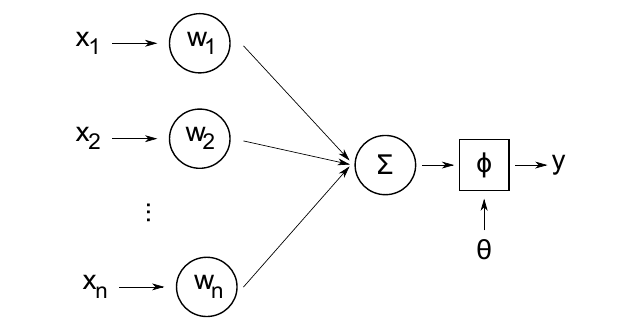
\includegraphics[scale=0.4]{perceptron.png}
% \label{single_layer}
% \caption{A single layer perceptron}
\end{center}

The activation function has to be fixed. The Heaviside function is commonly used and defined by:
\[H(x)= \begin{cases}
      0 & x< 0 \\
      1 & x\geq 0 
   \end{cases}
\]
This function is however discontinuous and thus implies more complexity during the learning step.\\
In machine learning, several functions are commonly used:
\begin{itemize}
 \item The logistic function:
$\displaystyle \sigma(x) = \frac{1}{1+e^{-x}}$
 \item The hyperbolic tangent function:
$\displaystyle \text{tanh}(x) = \frac{e^x - e^{-x}}{e^x+e^{-x}}$
\end{itemize}
These functions are implemented in the module.

A multi-layer perceptron consists of multiple layers of perceptrons, each neuron in a layer being connected to neurons of the previous layer.
Each layer also contains an activation function (which has the same properties as with single-layer perceptrons) and a bias.  The most commonly
used multi-layer perceptron is the 2-layer perceptron:
\begin{center}
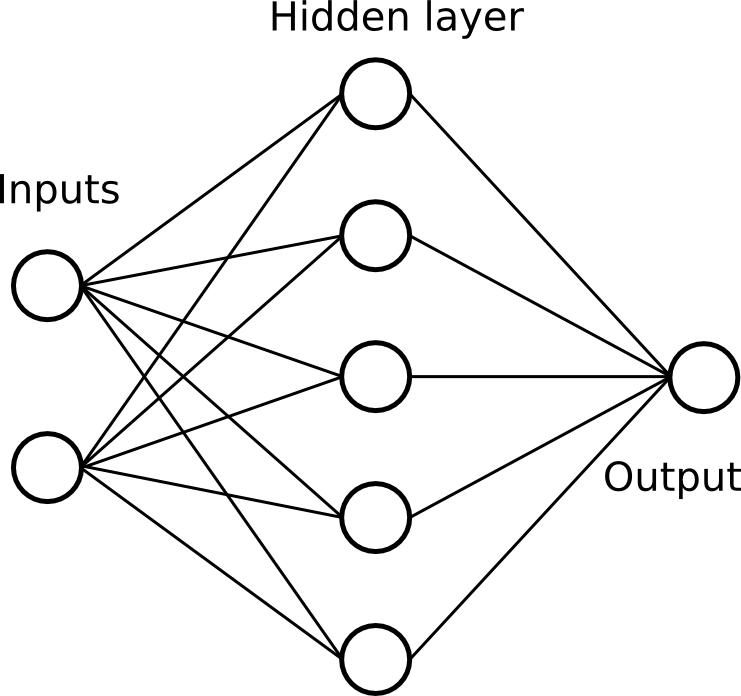
\includegraphics[scale=0.3]{single_layer.png}
\end{center}

If we note $(w,\theta,\phi)$ (resp. $(w^H,\theta^H,\phi^H)$) weights, bias and activation function of the output layer (resp. hidden layer), then
the expression of this neural network model, evaluated on the point of interest $x\in \mathbb{R}^n$, is given by:
\begin{eqnarray*}
\mathcal{M}(x) &=& \phi\left( \sum_{j=1}^M{w_j \mathcal{M}^H_j(x) - \theta} \right) \\
     &=& \phi\left[ \sum_{j=1}^M{w_j \phi^H\left(\sum_{k=1}^{M^H}{w^H_k x_k - \theta^H}\right) - \theta} \right] \\
\end{eqnarray*}

This can be generalized to any number of layers, but in practice a single hidden layer is sufficient.
}

{
% Autres notations et appellations
}

\Methodology{
This method is aimed at building a response surface prior to tackling Step C “Uncertainty Propagation”.
It requires an experimental design together with the corresponding model evaluations.
}
{

\vspace{1mm}

\begin{itemize}
\item Christopher M. Bishop 1995, ``Neural Networks for Pattern Recognition'', Oxford University Press, Inc, New York.
\end{itemize}
}

\subsection{Regression model}
\MathematicalDescription{
\underline{\textbf{Goal}}\\

The objectif is to evaluate a linear model regression issued from the \texttt{URANIE} platform.\\ 
  
\underline{\textbf{Principles}}\\

One considers global approximations of the model response using a polynomial of degree one:
\begin{align*}
  y \, \, \approx \, \, \widehat{h}(\underline{x}) \, \, = \, \, a_0 \, + \,  \sum_{i=1}^{n_{X}} \; a_{i} \; x_i
\end{align*}
where $(a_j  \, , \, j=0,\dots,n_X)$ is a set of unknown coefficients. \\

Several techniques are used to estimate the coefficients of the model.\\
In the propagation context, an experimental design $\underline{\mathcal{X}} =(x^{(1)},\dots,x^{(N)})$, i.e. a set of realizations of input parameters is required, as well 
as the corresponding model evaluations $\underline{\mathcal{Y}} =(y^{(1)},\dots,y^{(N)})$. Thus the coefficients $a_j$ may be computed using a least squares regression approach. \\

The following minimization problem has to be solved:
\begin{align*}
  \mbox{Find} \quad \widehat{\underline{a}} \quad \mbox{that minimizes} \quad \mathcal{J}(\underline{a}) \, \, = \, \, \sum_{i=1}^N \; \left( y^{(i)} \; - \; a_0 - \sum_{j=1}^{n_{X}} a_j \underline{x_{j}}^{(i)} \right)^2
\end{align*}

A necessary condition is that the size $N$ of the experimental design is not less than the number $n_{X}+1$ of coefficients to estimate. \\
%Over techniques may be investigated
}

{
% Autres notations et appellations
}

\Methodology{
Within the global methodology, the method is used to assess the accuracy of a polynomial response surface
of a model output prior to tackling the step C: <<Uncertainty propagation>>.

}
{
\vspace{1mm}
\begin{itemize}
\item {\AA}. Bjorck, 1996, ``Numerical methods for least squares problems'', SIAM Press, Philadelphia, PA.
\end{itemize}

}
